\paragraph{Methodology of the ENG subproject.}

\begin{figure}[h!]
\begin{center}
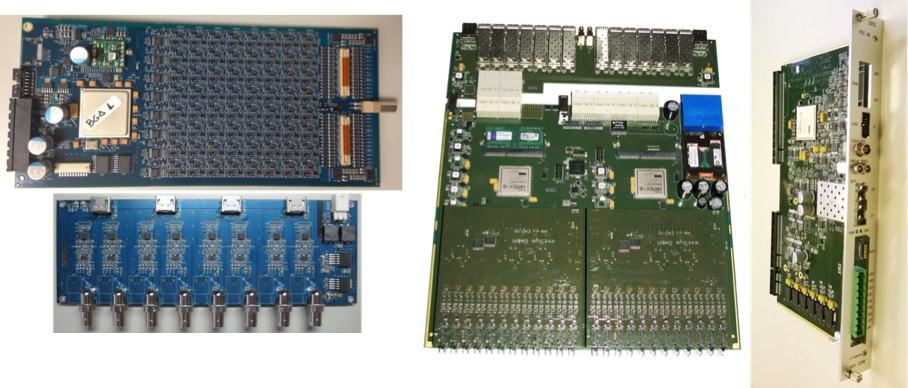
\includegraphics[width=0.7\textwidth]{img/Electronics.jpg}
\end{center}
\caption{\label{Fig:FEE}\small Left: Front-end boards for SiPM (top) and PMTs (bottom) for NEW and NEXT-100. Right: SRS FEC modules in ATCA form factor (left) and “SRS classic” flavour (right).}
\end{figure}

The ENG subproject is responsible for the {\bf front-end electronics} for the PMTs and the SiPMs for NEW and NEXT-100. Critical items include:
%
\begin{enumerate}
\item	{\em Commissioning NEW front-end electronics in 2015}. As an outcome from two previous projects (CUP and FIS2012-37947-C04-04), the front-end electronics for both the PMT plane and the SiPM plane in NEW are available. The former is already being used in NEXT-DEMO while the latter, an evolution from the NEXT-DEMO electronics, exists as prototype boards and will be available in adequate quantities by the end of 2014. Required cabling, power supplies and mechanical structures have already been purchased.
These electronics will be tested at IFIC in Q1’15 and at the LSC in Q2’15. A study on reliability, performance and signal noise will be carried out during the commissioning phase, resulting either on the final validation of the current designs or on a proposal for changes. In this case, the changes will be carried out in Q4’15 and Q1’16.

\item {\em Production, installation and test of NEXT-100 front-end electronics in 2016}. Lessons learnt with NEW commissioning and initial operation will lead to a document on recommendations for installation and operation of electronics in NEXT-100. The specificity of LSC in terms of grounding and power distribution in the experimental area, together from noise in the power lines and generated by neighbouring experiments, will determine the required noise-reduction techniques (mostly ground connections and ad-hoc filtering). After completing the eventual modifications in the front-end modules (Q1'15), production for NEXT-100 in Q2’16, and Q3'16, module test in Q4’16 will complete the 2016 work plan.

\item {\em Commissioning and Operation of NEXT-100 front-end electronics in 2017}. Potential problems found after installation in a detector of the size of NEXT-100 will be addressed. Front-end firmware may require fine adjustments to (1) ease later energy measurement and tracking algorithms and (2) adjust the trigger algorithms as specified for the different physics campaigns. Commissioning is scheduled for Q1-Q2’17. Operations start on the second half of the year.
\end{enumerate}

%%%%%%%%%%%%%%%%%%%%%%

The second objective of this subproject is the design, fabrication and commissioning of the {\bf data acquisition modules} for NEW and NEXT-100. The following main tasks have been identified:

\begin{enumerate}

\item	{\em Commissioning NEW DAQ interface electronics in 2015}. The DAQ interface modules for NEW and NEXT-100 are also available in two flavours: “classic” SRS modules (19” Eurocard form factor, available from CERN Store) and industry-standard ATCA SRS modules. NEW DAQ will use in a first stage modules from both flavours.

These electronics will be tested at IFIC in Q1’15 and at LSC in Q2’15. A study on reliability and performance will be carried out during the commissioning phase, allowing to choose the best solution for NEW and NEXT-100. 
%A third option, a new SRS solution for very-close-to-detector readout codenamed OC-Box, which is to be developed in collaboration with RD51 and intended as an upgrade for NEXT, will be evaluated in 2015 as a future upgrade. It is based on newer FPGA technology and can replace current FEC modules.

\item	{\em Production, installation and test of NEXT-100 DAQ electronics in 2016}. Lessons learnt with NEW commissioning and initial operation will lead to a decision to go for “classic” or ATCA SRS flavor. Purchases for NEXT-100 in Q2’16, module test and firmware upgrade in Q3’16 and installation in Q4’16 will complete the 2016 work plan.

\item	{\em Commissioning and Operation of NEXT-100 DAQ electronics in 2017}. DAQ performance and functionalities will be verified and adjusted to meet final NEXT-100 requirements. DAQ firmware may require some modifications to (1) ease energy measurement and tracking algorithms and (2) adjust the trigger algorithms as specified.

%\item	NEXT-100 operation in 2018. The DAQ requires no maintenance during operation other than module replacement due to damage or malfunctioning. Placed outside the lead castle in 19” racks next to the front-end modules, the DAQ electronics are easily accessible.

\end{enumerate}

%%%%%%%%%%%%%%%%%%%%%%

Concerning the third objective of the ENG subproject, the {\bf slow controls system} for NEW and NEXT-100, six subsystems or partitions have been defined: (1) high-voltage sources for PMTs, (2) low-voltage sources for SiPMs and electronics, (3) high-voltage for grids, (4) gas system status -getters, pump and gas recirculation-, (5) a group of temperature and pressure sensors and (6) the main control panel (with cameras and status overview). Partitions are interconnected via Ethernet. Basic functionalities for all subsystems have been implemented in 2014. The Slow Controls for NEW will be completed in Q4’14, tested and debugged in Q1’15 and installed in LSC in Q2’15.

%Power supplies for PMTs and SiPMs are directly controlled to Ethernet. Power supplies for the electronics are controller from a PC via USB, being this PC connected to Ethernet. The other subsystems are controlled via a National Instrument’s Compact-RIO chassis with Ethernet link, embedded in a so-called “Slow Control Box”, which includes relays and connections. A LabView software application will be used for the main control panel.

%\begin{enumerate}
%\item {\em Design, production and commissioning NEW slow-controls in 2015}. The Slow Controls for NEW will be completed in Q4’14, tested and debugged in  Q1’15 and installed in LSC in Q2’15.

%\item {\em Production, installation and commissioning of NEXT-100 slow-controls electronics}. Monitoring the gas subsystem will be an addition to the Slow Controls for NEXT-100 in 2016.
%\end{enumerate}

%%%%%%%%%%%%%%%%%%%%%%

Finally, the ENG subproject is respnsible for the {\bf online system} for NEW and NEXT-100. The Online System for NEW comprises the following subsystems: (1) Data Storage, (b) Backup Storage, (c) Pre-processing and (d) Online Monitoring. The DAQ System (a PC farm comprising Local and Global Data Concentrators) produces approx. 30 MByte/s in NEW, which are stored into the NEW Data Storage (up to 8 servers with 8 disks each for up to 65 TByte). The Data Storage has power redundancy and multiple network cards per PC for enhanced reliability. Long-term data selected by the Offline System are stored into the Backup Storage (composed of a server PC and a tape server using 1.5 TByte tapes). The Pre-processing comprises two servers which read event data from the Data Storage and apply a format for later offline processing. Finally, a server in the Online Monitoring is used to gather statics, measure performance, find out bottlenecks and check the health of the different subsystems. A 1-Gb Ethernet switch interconnects the PC servers in the Online System, using virtual LANs to separate different data flows.
Backup Storage, Pre-Processing, Data Storage and Online Monitoring have been tested.
